В первом задании займёмся фильтрацией изоображения под номером 8, приведенного ниже:
\vspace{1cm}
\begin{figure}[ht!]
    \centering
    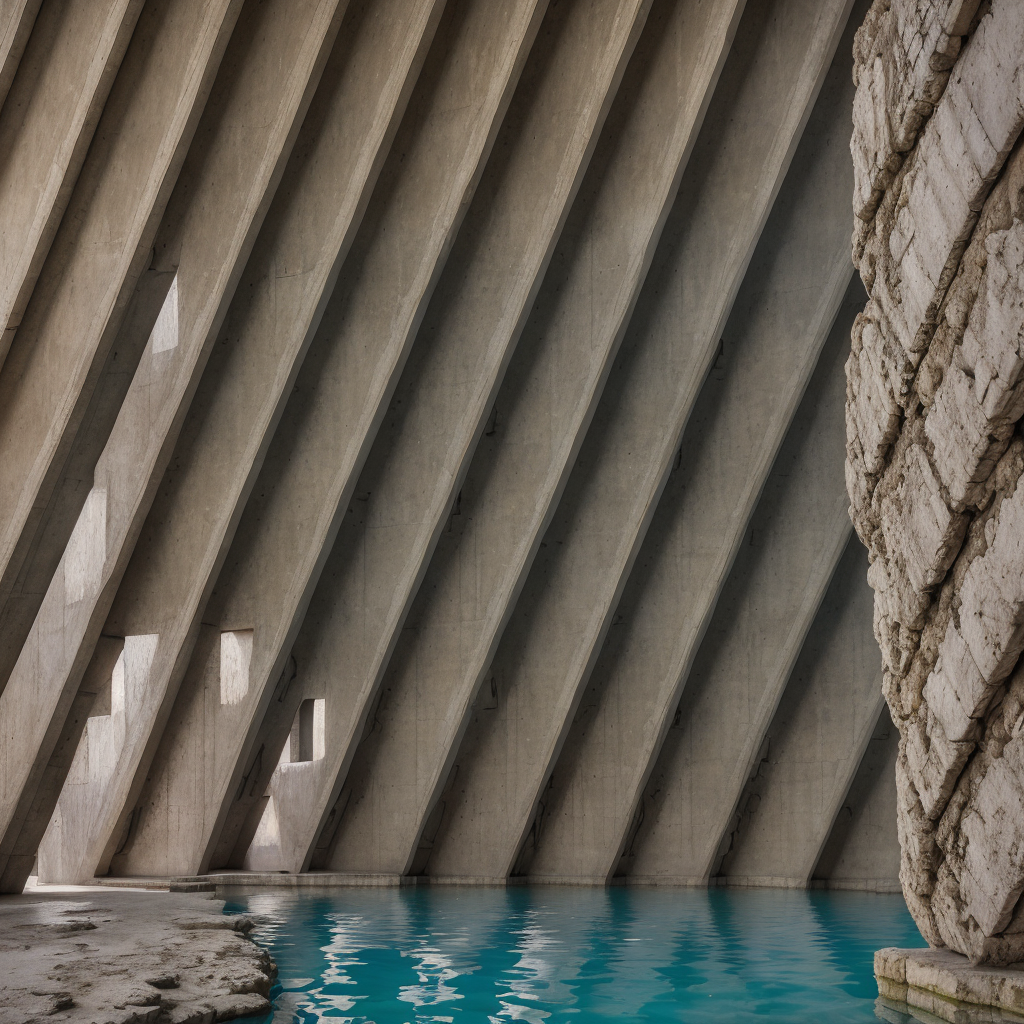
\includegraphics[width=0.95\textwidth]{images/source_images/task_1/8.png}
    \caption{Изображение 8 -- Бэтпещера нормального человека}
    \label{fig:photo_8}
\end{figure}
\clearpage
Найдём логарифм модуля сдвинутого Фурье-образа:
\vspace{1.5cm}
\begin{figure}[ht!]
    \centering
    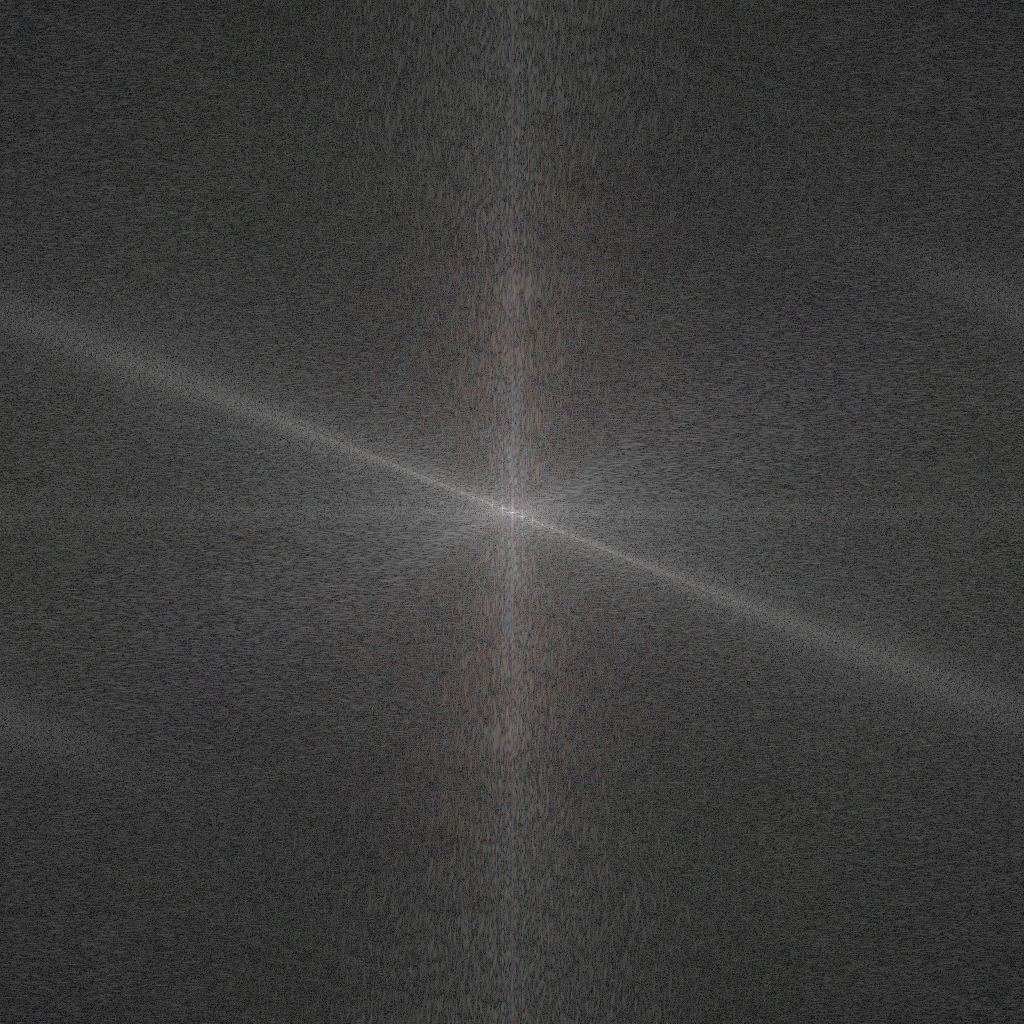
\includegraphics[width=0.95\textwidth]{images/result/task_1/Fourier_8.png}
    \caption{Логарифм модуля сдвинутого Фурье-образа}
    \label{fig:image_8}
\end{figure}
\vspace{1cm}

Помимо центрального пика, на изображении отчётливо видны 8 пиков.
\clearpage
\begin{figure}[ht!]
    \centering
    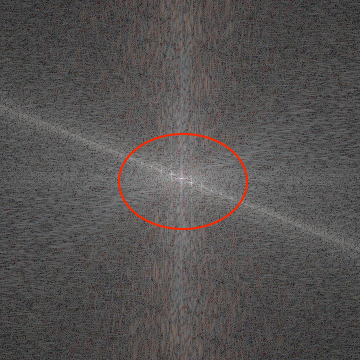
\includegraphics[width=0.6\textwidth]{images/result/task_1/Fourier_8_peaks.png}
    \caption{Цветовые пики, соответствующие гармоникам}
    \label{fig:image_8_peaks}
\end{figure}

Будем последовательно закрашивать каждую пару пиков. Начнём с самой яркой пары:

\begin{figure}[ht!]
    \centering
    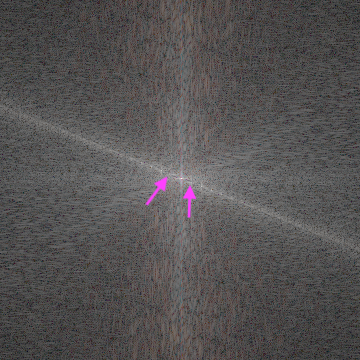
\includegraphics[width=0.6\textwidth]{images/result/task_1/Fourier_8_modified_1_peaks.png}
    \caption{Образ Фурье после удаления двух пиков}
    \label{fig:image_8_m1}
\end{figure}

\vspace{2cm}

\begin{figure}[ht!]
    \centering
    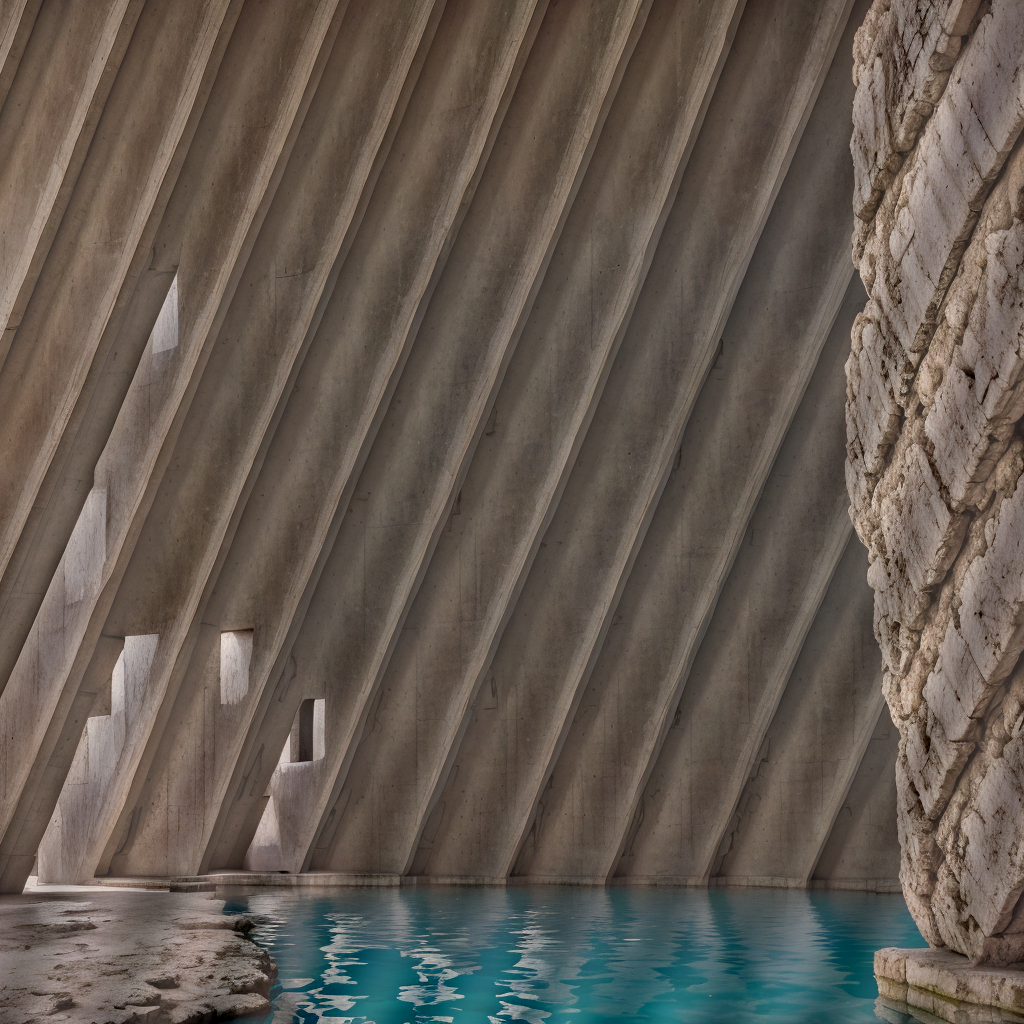
\includegraphics[width=0.95\textwidth]{images/result/task_1/result_8_1.png}
    \caption{Изображение после удаления двух пиков}
    \label{fig:photo_8_m1}
\end{figure}

Изображение стало более блеклым, на нём появились темно-серые полосы, особенно это заметно на бетонных столбах и скалах. При этом темные участки (пространство между столбами). Это связано с тем, что светлые пики на образе были закрашены серыми пикселями (рис. \ref{fig:image_8_m1}).

Теперь закрасим следующую пару пиков:


\begin{figure}[ht!]
    \centering
    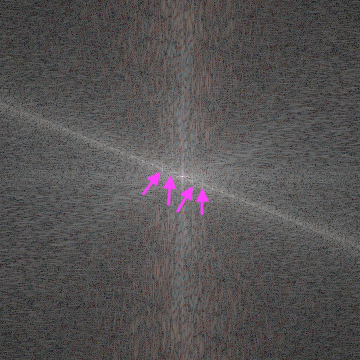
\includegraphics[width=\textwidth]{images/result/task_1/Fourier_8_modified_2_peaks.png}
    \caption{Образ Фурье после удаления четырех пиков}
    \label{fig:image_8_m2}
\end{figure}
\clearpage
\begin{figure}[ht!]
    \centering
    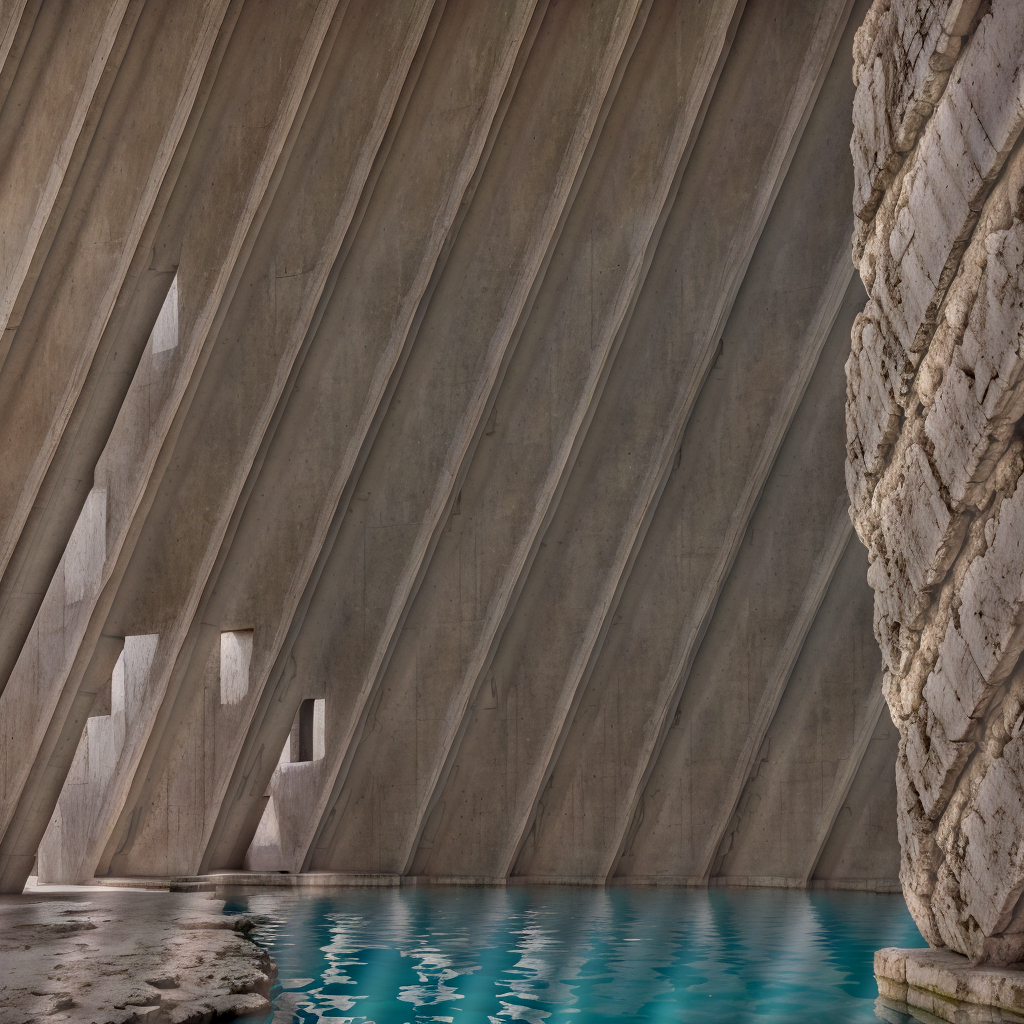
\includegraphics[width=0.95\textwidth]{images/result/task_1/result_8_2.png}
    \caption{Изображение после удаления четырех пиков}
    \label{fig:photo_8_m2}
\end{figure}

Полосы на изображении стали шире и более блеклыми, темные области между столбами -- светлее. 

Далее закрасим все пики на Фурье-образе:

\begin{figure}[ht!]
    \centering
    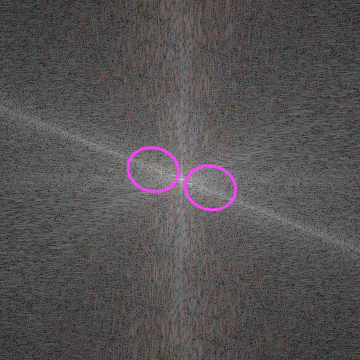
\includegraphics[width=\textwidth]{images/result/task_1/Fourier_8_modified_3_peaks.png}
    \caption{Образ Фурье после удаления восьми пиков}
    \label{fig:image_8_m3}
\end{figure}
\clearpage
\begin{figure}[ht!]
    \centering
    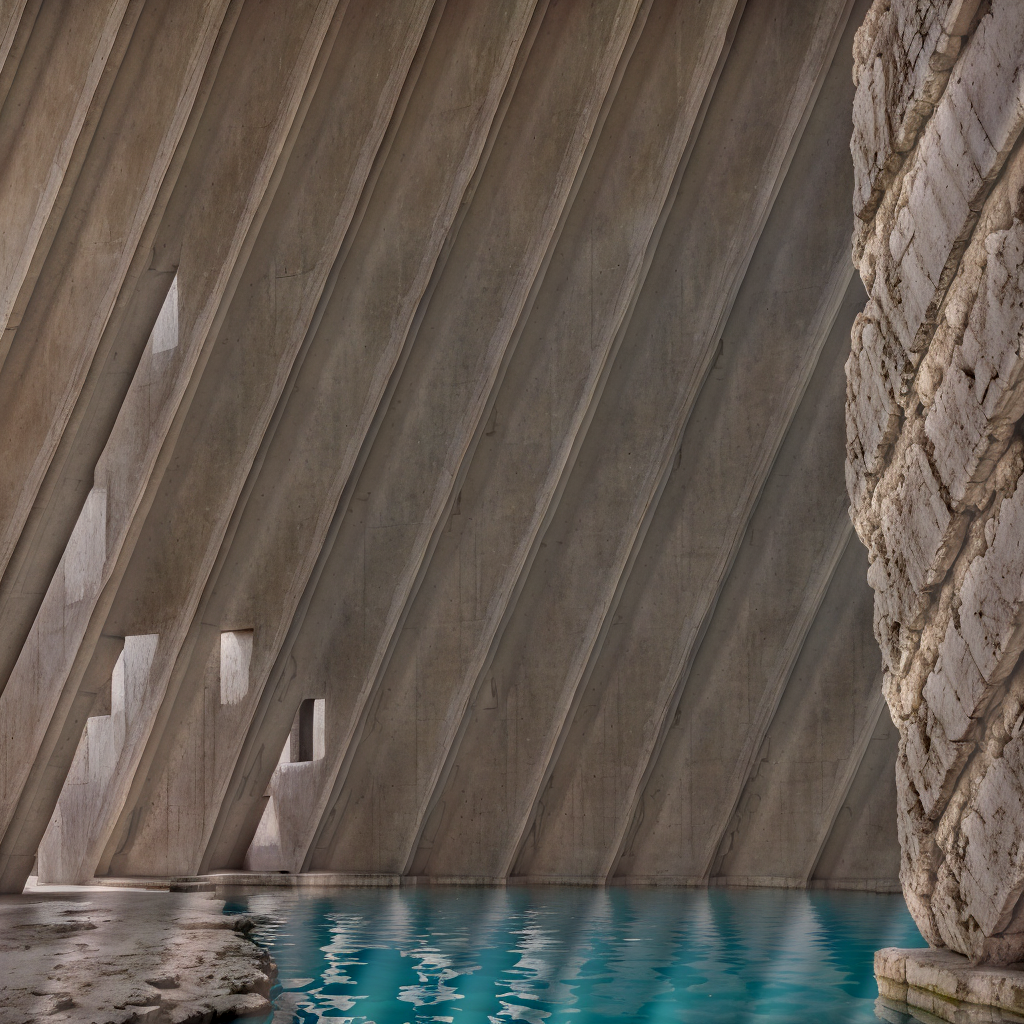
\includegraphics[width=0.95\textwidth]{images/result/task_1/result_8_3.png}
    \caption{Изображение после удаления восьми пиков}
    \label{fig:photo_8_m3}
\end{figure}
Полученное изображение стало менее контрастным по сравнению с предыдущими. 

Обращаясь к исходному изображению (рис. \ref{fig:photo_8}), полученные фотографии выглядят менее красочными и объёмными: бетонные столбы <<слиплись>>, став одной стеной. В целом полученные изображения выглядят неестественно: на поверхности воды появились темные полосы, на скале темные и светлые области поменялись местами.
